%%%%%%%%%%%%%%% PLEASE NOTE THE FOLLOWING STYLE RESTRICTIONS %%%%%%%%%%%%%%%
%%
%%  1. There are no new tags.  Existing LaTeX tags have been formatted to match
%%     the Preprint series style.    
%%
%%  2. You must use \cite in the text to mark your reference citations and 
%%     \bibitem in the listing of references at the end of your chapter. See
%%     the examples in the following file. If you are using BibTeX, please
%%     supply the bst file with the manuscript file.
%% 
%%  3. This macro is set up for two levels of headings (\section and 
%%     \subsection). The macro will automatically number the headings for you.
%%
%%  5. No running heads are to be used for this volume.
%% 
%%  6. Theorems, Lemmas, Definitions, etc. are to be double numbered, 
%%     indicating the section and the occurence of that element
%%     within that section. (For example, the first theorem in the second
%%     section would be numbered 2.1. The macro will 
%%     automatically do the numbering for you.
%%
%%  7. Figures, equations, and tables must be single-numbered. 
%%     Use existing LaTeX tags for these elements.
%%     Numbering will be done automatically.
%%   
%%%%%%%%%%%%%%%%%%%%%%%%%%%%%%%%%%%%%%%%%%%%%%%%%%%%%%%%%%%%%%%%%%%%%%%%%%%%%%%



\documentclass[twoside,leqno,twocolumn]{article}
\usepackage{ltexpprt, amsmath, amssymb, graphicx}

\DeclareMathOperator{\kda}{kda}
\DeclareMathOperator{\multi}{multi}

\newcommand{\x}{\\~~}
\newcommand{\xx}{\\~~~~}
\newcommand{\xxx}{\\~~~~~~}
\newcommand{\xxxx}{\\~~~~~~~~}
\newcommand{\xfunction}{{\bf function}\:}
\newcommand{\xinit}{{\bf init}\:}
\newcommand{\xlet}{{\bf let}\:}
\newcommand{\xif}{{\bf if}\:}
\newcommand{\xelif}{{\bf elif}\:}
\newcommand{\xelse}{{\bf else}\:}
\newcommand{\xfor}{{\bf for}\:}
\newcommand{\xeach}{{\bf each}\:}
\newcommand{\xreturn}{{\bf return}\:}
\newcommand{\xbreak}{{\bf break}\:}
\newcommand{\xcontinue}{{\bf continue}\:}

\newcommand{\peq}{\mathbin{\mathord{+}\mathord{=}}}

\newcommand{\kdroot}[1]{#1^{\rm root}}
\newcommand{\kdleft}[1]{#1^{\!L}}
\newcommand{\kdright}[1]{#1^{\!R}}
\newcommand{\lo}[1]{#1^{\,l}}
\newcommand{\hi}[1]{#1^u}
\newcommand{\lohi}[1]{#1^{l,u}}

\newcommand{\leftlim}[1]{\lefteqn{\scriptscriptstyle #1}}

\begin{document}

%\setcounter{chapter}{2} % If you are doing your chapter as chapter one,
%\setcounter{section}{3} % comment these two lines out.

\title{\Large Massive-Scale Kernel Discriminant Analysis: Mining for Quasars\thanks{We would also like to acknowledge the contributions of astrophysicists Robert Nichol and Robert Bruner}}
\author{Ryan Riegel\thanks{Georgia Institute of Technology.} \\
  \and Alexander Gray\thanks{Georgia Institute of Technology..} \\
  \and Gordon Richards\thanks{Johns Hopkins University.}}
\date{}

\maketitle

%\pagenumbering{arabic}
%\setcounter{page}{1}%Leave this line commented out.

\begin{abstract} \small\baselineskip=9pt
  We describe a fast algorithm for kernel discriminant analysis,
  empirically demonstrating asymptotic speed-up over the previous best
  approach.  We achieve this with a new pattern of processing data
  stored in hierarchical trees, which incurs low overhead while
  helping to prune unnecessary work once classification results can be
  shown, and the use of the Epanechnikov kernel, which allows
  additional pruning between portions of data shown to be far apart or
  very near each other.  Further, our algorithm may share work between
  multiple simultaneous bandwidth computations, thus facilitating a
  rudimentary but nonetheless quick and effective means of bandwidth
  optimization.  We apply a parallelized implementation of our
  algorithm to a large data set (40 million points in 4D) from the
  Sloan Digital Sky Survey, identifying approximately one million
  quasars with high accuracy.  This exceeds the previous largest
  catalog of quasars in size by a factor of ten.
\end{abstract}

{\bf Keywords:} Kernel Discriminant Analysis, Scalable Algorithm, Classification, Bandwidth Learning, Astrophysics

\section{Classification Via Density Estimation}
Kernel discriminant analysis (KDA) \cite{fix-hodges}, also called
kernel density classification \cite{hastie-tib-frie} or nonparametric
Bayes classification, is a nonparametric method for predicting the
class of query observations given a set of labeled reference
observations.  It is particularly useful in scientific applications
due to its balance of properties:
\begin{enumerate}
\item It is highly accurate, owing to its nonparametric form.
\item It is easy to use in that it requires little understanding of
  the problem's underlying model but still offers an intuitive means
  of incorporating prior knowledge.
\item If desired, its classifications are also accompanied by highly
  accurate probabilities of inclusion in each class, which can be
  useful in their own right.
\end{enumerate}

We are motivated by a high-profile application in astrophysics
pertaining to the identification of quasars.  Believed to be active
galactic nuclei, quasars are the brightest objects in the universe,
typically out-shining their entire host galaxy by several orders of
magnitude.  As a result, they are the most distant and thus oldest
objects we can see, making knowledge of their locations invaluable to
the verification of theories such as dark energy.  Prior to work with
our astrophysicist collaborators \cite{richards04}, the largest
available catalog of quasars listed fewer than one hundred thousand
examples; massive sky surveys such as the Sloan Digital Sky Survey
(SDSS), on the other hand, are expected to contain millions.  Our goal
is then to predict which of the unlabeled objects in the survey are
quasars given a comparatively small (though still prohibitively large)
sample of hand-identified objects.

Until recently, there was no feasible means of performing exact KDA
when both the number of queries and number of references were large;
traditionally, KDA is $O(N^2)$ when there are $O(N)$ queries and
$O(N)$ references.  Further, existing approximate methods do not
provide hard bounds on introduced error.  A new algorithmic approach
presented in \cite{nbc-compstat}, however, offers marked improvement
to running-time with {\em no} introduction of error.  In this paper,
we describe a new algorithm similar to that of \cite{nbc-compstat}
which achieves dramatic asymptotic speed-up.

The remainder of this section details the mathematics of KDA.
Following that, we examine what it takes to make a fast algorithm for
KDA, juxtaposing previous work with the primary contributions of this
paper.  Sections~\ref{sec:math} and~\ref{sec:alg} establish a
framework for our algorithm and subsequently fill in the details.
Section~\ref{sec:bw} then considers accelerations to KDA's learning
phase and Section~\ref{sec:para} discusses the possibility of
parallelization.  In Section~\ref{sec:res}, we demonstrate our
algorithm's superior performance on two data sets.

\subsection{Bayes' Rule in Classification.}
Bayes' rule,
\begin{equation}
  P(A|B) = \frac{P(B|A)P(A)}{P(B)} ,
\end{equation}
is a fundamental relationship between prior and posterior
probabilities used in a wide variety of statistical methods.  As shown
in \cite{rao73}, the optimal classifier on $M$ classes assigns observation
$x \in \mathcal{X}$ to the class $C_k$ with the greatest posterior
probability $P(C_k|x)$.  Applying Bayes' rule, we assign $x$ to $C_k$
if, for all $l \neq k$, $1 \leq l \leq M$, we have
\begin{equation}\label{eqn:ineq-form}
  f(x|C_k)P(C_k) > f(x|C_l)P(C_l) ,
\end{equation}
where $f(x|C)$ denotes the probability density of data sampled from
$C$ and $P(C)$ is the prior probability of $C$.  (Note that Bayes'
rule's denominator $f(x)$ cancels from either side.)  It is typically
given that $\sum_{k=1}^M P(C_k) = 1$, i.e.~that there are no
unexplained classes, and accordingly, that $f(x) = \sum_{k=1}^M
f(x|C_k)P(C_k)$.  In the case that $M = 2$, this implies that it is
equivalent to classify $x$ as $C_1$ when $P(C_1|x) =$
\begin{equation}\label{eqn:prob-form}
  \frac{f(x|C_1)P(C_1)}{f(x|C_1)P(C_1) + f(x|C_2)P(C_2)} > 0.5 .
\end{equation}

\subsection{Kernel Discriminant Analysis.}
In place of the typically unknown values of $f(x|C)$, KDA uses kernel
density estimates of the form
\begin{equation}
  \widehat{f}_h(x|C) = \frac{1}{N} \sum_{i=1}^N K_h(x,z_i) ,
\end{equation}
trained with bandwidth $h$ on a size $N$ set of reference observations
$z_i \in \mathcal{X}$ of class $C$.  Kernel $K_h$ may take many forms
but must be non-negative and have
\begin{equation}
  \int_{\mathcal{X}} K_h(x,z) dx = 1
\end{equation}
for all $z$, i.e.~it must be a probability density function.  For
$\mathcal{X} = \mathbb{R}^D$, a popular choice of kernel is the
Gaussian,
\begin{equation}
  K_h(x,z) = \frac{1}{\left( h \sqrt{2 \pi} \right)^D} \exp \! \left( \frac{- \| x - z \|^2}{2 h^2} \right) ,
\end{equation}
though \cite{silverman86} shows that the optimal kernel for density
estimation is in fact the Epanechnikov kernel,
\begin{equation}
  K_h(x,z) = \max \left\{ \frac{D + 2}{2 V_D(h)} \left( 1 - \frac{\| x - z \|^2}{h^2} \right), 0 \right\} ,
\end{equation}
where $V_D(h)$ is the volume of a $D$-dimensional sphere with radius
$h$.  Observe that the Epanechnikov kernel is a parabolic function of
distance for $\| x - z \| < h$ and zero otherwise; we will later
exploit this property to accelerate computation.  Also, note that many
kernels are actually functions of distance $d(x,z) = \| x - z \|$;
later in this paper, $K_h$ of one argument is understood to work on
the distance term directly.

Proper selection of bandwidths $h_k$, $1 \leq k \leq M$, is critical
for accurate classification results.  \cite{silverman86} provides some
theoretical insights on how a data set's variance and size should
inform bandwidth choice, but in practice, it is most effective to
choose bandwidths that minimize cross-validation error or some other
measure of loss.

\subsection{Extensions to the Classifier.}
It is not uncommon to have additional information $y \in \mathcal{Y}$
available for each observation $x$ that is nonetheless difficult to
incorporate into density estimates $\widehat{f}_h(x|C)$.  For
instance, corresponding information in $\mathcal{Y}$ may not be
available for all of the references, or $\mathcal{Y}$ may not be
favorable to kernels (e.g.~may have no workable interpretation as
$\mathbb{R}^D$).  If it is reasonable to assume that $y$ has
negligible effect on class-conditional densities, we may still capture
its effect in the class' priors with
\begin{equation}
  P(C|x,y) \propto f(x|C,y)P(C|y) \approx f(x|C)P(C|y) .
\end{equation}
Similarly, for fine-tuned control over density estimates, we may
provide weight $w_i$ with each reference $z_i$, giving
\begin{equation}
  \widehat{f}_h(x|C) = \sum_{i=1}^N w_i K_h(x,z_i) ,
\end{equation}
where $\sum_{i=1}^N w_i = 1$.

Another modification possible in the $M = 2$ case replaces the $0.5$
in (\ref{eqn:prob-form}) with an alternate confidence threshold $t$.
Rather than performing optimal classification, this has the effect of
identifying points with very high (or low) probability of being in
$C_1$, which can be a useful surrogate for fully computed class
probabilities.  Simple algebra and incorporation of the above gives us
\begin{equation}\label{eqn:thresh-form}
  (1 - t)\widehat{f}_{h_1}(x|C_1)P(C_1|y) > t\widehat{f}_{h_2}(x|C_2)P(C_2|y) ;
\end{equation}
we will use this as our classification test for the remainder of this
paper.  This modification may seem trivial from the mindset of
na\"{\i}ve computation, which provides exhaustively computed class
probabilities for each query, but it is useful under the new
algorithmic approach.  Our algorithm deals only in bounds on
probabilities and aims to terminate computation on a query as soon as
it is possible to demonstrate (\ref{eqn:thresh-form}) or its converse.
While we will know that the query's probability is definitely above or
below the threshold, we have no guarantee of being able to show by how
far.

\section{Computational Considerations}
An obvious means of performing KDA is to compute the full kernel
summation for each query.  For $O(N)$ queries and $O(N)$ references,
this na\"{\i}ve algorithm is $O(N^2)$ overall.  While this approach is
trivial to implement even in parallel, it does not scale to large $N$.
In the best of conditions, a compute cluster with ten thousand nodes
would only be able to handle a problem two orders of magnitude larger
than is feasible on a single machine.

In order to make asymptotic improvement to running time, it is
necessary to avoid a great deal of the explicit kernel evaluations.  A
new computational approach developed in \cite{nbc-compstat} achieves this by
rearranging work in a manner that permits consideration of subsets of
queries and references at an abstract level.  It is then hoped that
bounds on results obtained at abstract levels can demonstrate that
further work is unnecessary and can thus be {\em pruned}.  For
example, as suggested above, we may prune all remaining work on a
subset of queries if density bounds prove (\ref{eqn:thresh-form}) or
its converse for each of the queries.

\subsection{Previous Work.}
The algorithm presented in \cite{nbc-compstat} is best described as a
high-order divide-and-conquer method for the $M = 2$ case of KDA.  In
a nutshell, it constructs two binary spatial trees, one on the query
data and one on the reference data, with pairs of nodes from either
tree representing abstracted computations.  It then iteratively
refines bounds on class-conditional density estimates
$\widehat{f}_{h_1}(x|C_1)$ and $\widehat{f}_{h_2}(x|C_2)$ until each
query's classification can be shown.  Given bounding boxes for either
node in a pair, bounds on the pair's contribution to densities are
computed using kernel evaluations at the pair's minimum and maximum
distances.  Bounds are refined by, at each iteration, heuristically
selecting an unrefined pair and replacing its contribution with the
combined contributions of its four child pairs.  If
(\ref{eqn:thresh-form}) becomes provably true or false for a query
node, i.e.~one class' lower-bound probability becomes greater than the
other's upper-bound probability, then the queries represented by the
node are appropriately labeled and further work on those queries is
removed from consideration.  Ideally, bounds give a query's
classification long before all references are visited exhaustively,
thereby abbreviating computation while still yielding the exact
result.

\subsection{This Paper.}
In this paper, we directly extend the work done in
\cite{nbc-compstat}.  Our new algorithm is the same in spirit as the
old one and is also implemented specifically\footnote{Though no
inherent properties of the algorithm prevent it from being extended to
$M > 2$.} for $M = 2$, but it benefits from several key differences:
\begin{itemize}
\item It uses an improved work order that better favors pruning and is
  implemented with reduced overhead and improved numerical stability.
\item It uses the Epanechnikov kernel, which enables a new kind of
  pruning based on bounded distances between node pairs.
\item It can compute results for multiple bandwidth combinations
  simultaneously, sharing work to accelerate bandwidth optimization.
\item It can parallelize computation over the queries, making use of
  spatial information to reduce each processor's overall workload.
\end{itemize}
We achieve empirically asymptotic improvement over the previous best
algorithm, met with multiple orders of magnitude improvement on the
data sets we examined.

\section{Foundations}\label{sec:math}
Previous work \cite{nbc-compstat} does not formalize the manner of
rearranging work it uses to make efficient computation possible.  We
include the underlying mathematics here for the purposes of rigor and
helping to clarify how the algorithm presented in this paper works.

In all of the following, $X$ is a subset of the full query set
$\kdroot{X} \subset \mathcal{X} \times \mathbb{R}$.  Queries are given
by pairs $(x,\pi)$, where $x$ is used in density estimation and $\pi =
P(C_1|y)$.  Symbol $Z_k$ represents a subset of the weighted
references $\kdroot{Z_k} \subset \mathcal{Z} \times \mathbb{R}$
available for for class $C_k$.  References are pairs $(z,w)$, where
$z$ is used in kernel computations and $w$ is the weight.  Note that
the sum of weights of $\kdroot{Z_k}$ equals $1$, but the same of $Z_k$
generally does not.  We use ``root'' to denote full sets because they
are semantically equivalent to the roots of trees used by our
algorithm.

\subsection{Recursive Formulation.}
We represent density estimation with a set of key-value pairs
$\phi_k(X,Z_k)$, where
\begin{equation}
  \phi_k(X,Z_k) = \left\{ \!\! \left. \left( x, \sum_{\leftlim{(z,w) \in Z_k}} w K_{h_k}(x,z) \right) \right|
(x,\pi) \in X
  \right\} .
\end{equation}
Classification is then a task of comparing density estimates for
matching keys in $\phi_1(X,Z_1)$ and $\phi_2(X,Z_2)$ in accordance with
(\ref{eqn:thresh-form}).

For partitions $\kdleft{X} \cup \kdright{X} = X$ and $\kdleft{Z_k} \cup
\kdright{Z_k} = Z_k$, observe that
\begin{align}
  \label{eqn:q-split} \phi_k(X,Z_k) & = \phi_k(\kdleft{X},Z_k) \cup \phi_k(\kdright{X},Z_k) \\
  \label{eqn:r-split} & = \phi_k(X,\kdleft{Z_k}) + \phi_k(X,\kdright{Z_k}) ,
\end{align}
where addition on sets of key-value pairs is understood to add values
for matching keys.  This immediately suggests a recursive alternative
to the na\"{\i}ve algorithm in which the query set and reference sets
are repeatedly split until they become singleton, whereupon $\phi_k$ may
be computed directly.  Note that this reformulation by itself does
nothing to help asymptotic running time because, without pruning, each
of the $O(N^2)$ kernel evaluations will ultimately occur.  What it
does offer is the occurrence of $\phi_k(X,Z_k)$ for (generally)
nontrivial subsets $X \subseteq \kdroot{X}$ and $Z_k \subseteq
\kdroot{Z_k}$, instrumental to bounds computation and pruning.

Our algorithm cannot afford to spend much time deciding splits
$\kdleft{X} \cup \kdright{X} = X$, etc., so we use space partitioning
trees to decide these splits in advance.  This has the effect of
forcing the same partitions to occur throughout computation, though
this is not necessary in the underlying math.

\subsection{Bounds Computation.}
It is typically possible to bound kernel results between points in $X$
and $Z_k$ if we know bounding boxes or bounding radii for these sets.
In the case of the Gaussian and Epanechnikov kernels, bounds are
functions of upper- and lower-bound distances $\hi{d}(X,Z_k)$ and
$\lo{d}(X,Z_k)$ between the regions containing $X$ and $Z_k$, with
\begin{equation}
  \hi{K_{h_k}}(X,Z_k) = K_{h_k}(\lo{d}(X,Z_k))
\end{equation}
and vice versa.  Bounded contributions to density then assume that all
references are either maximally near to or maximally far from the
queries, and are given by
\begin{equation}
  \hi{\phi_k}(X,Z_k) = W(Z_k) \hi{K_{h_k}}(X,Z_k)
\end{equation}
and similarly for $\lo{\phi_k}(X,Z_k)$, where
\begin{equation}
  W(Z_k) = \sum_{\leftlim{(z,w) \in Z_k}} w .
\end{equation}
Note that bounds have zero width when $X$ and $Z_k$ are singleton and
are thus equivalent to exact computation.

To make use of these bounds in classification, we must compose them to
form bounds on the full density estimate, i.e.~such that they bound a
kernel summation over the full reference set.  For a query $(x,\pi)
\in X$, this is achieved by combining the bounds of $P$ components of
computation with
\begin{equation}\label{eqn:dens-bds}
  \hi{\Phi_k}(x) \gets \sum_{p=i}^{P} \hi{\phi_k}(X^p,Z_k^p)
\end{equation}
and similarly for $\lo{\Phi_k}(x)$, where $Z_k^p$, $1 \leq p \leq P$,
forms a partition of $\kdroot{Z_k}$ and $(x,\pi) \in X^p$ for each
$p$.  We further define
\begin{equation}
  \hi{\Phi_k}(X) \gets \max_{\leftlim{(x,\pi) \in X}} \hi{\Phi_k}(x) , \quad \lo{\Phi_k}(X) \gets \min_{\leftlim{(x,\pi) \in X}} \lo{\Phi_k}(x) ,
\end{equation}
which can be computed directly if $X \subseteq X^p$ for all $p$.

\subsection{Iterative Refinement.}
Computation under the new algorithmic approach implicitly constructs
two binary expression trees, one for either class, in accordance with
the recursive formulation given in (\ref{eqn:q-split}) and
(\ref{eqn:r-split}).  The nodes of these trees represent partial
density estimations $\phi_k(X,Z_k)$, with interior nodes symbolically
composing their children via $\cup$ or $+$.  Operation begins with
trees initialized to single nodes for
$\phi_1(\kdroot{X},\kdroot{Z_1})$ and
$\phi_2(\kdroot{X},\kdroot{Z_2})$, and at each iteration {\em expands}
a selected, non-singleton leaf into two children reflecting having
split either its queries or references.  After expansion, the
algorithm reassesses bounds on the full density estimates for the
involved queries as in (\ref{eqn:dens-bds}), using bounded results
computed for the newly created leaves in conjunction with bounds
already available from other leaves.\footnote{It is easy to prove by
induction that, for any $(x,\pi) \in X$, we can find leaves that satisfy
the requirements of (\ref{eqn:dens-bds}).}  We stop expanding nodes
$\phi_k(X,Z_k)$ for which we can show either of
\begin{align}
  \label{eqn:bd-form1} (1-t)\lo{\Phi_1}(X)\lo{\Pi}(X) > t\hi{\Phi_2}(X)(1-\lo{\Pi}(X)) , \\
  \label{eqn:bd-form2} t\lo{\Phi_2}(X)(1-\hi{\Pi}(X)) > (1-t)\hi{\Phi_1}(X)\hi{\Pi}(X) ,
\end{align}
where
\begin{equation}
  \hi{\Pi}(X) = \max_{\leftlim{(x,\pi) \in X}} \pi , \quad \lo{\Pi}(X) = \min_{\leftlim{(x,\pi) \in X}} \pi ,
\end{equation}
which decides (\ref{eqn:thresh-form}) for all queries in $X$.

It is easy to see that this procedure terminates.  For finite $X$ and
$Z_k$, recursion will ultimately reach singleton sets $X = \{x\}$ and
$Z_k = \{x_k\}$, where upon contribution bounds computations become
exact, i.e.~the upper and lower bound become equal, and recursion
along that branch ceases.  If all branches for some $x$ reach
singleton leaves, then bounds on the full density estimate are also
exact and thus one of (\ref{eqn:bd-form1}) or (\ref{eqn:bd-form2})
must be true\footnote{Or either side is exactly equal, but this is
degenerate and may be thought of as a third, nonclassifying prune.}
for each singleton $X$.  If branches do not reach leaves then it is
only because $x$ has already been pruned.  Thus, all queries $x$ will
eventually prune and iterative refinement will stop.  Correctness is
more difficult to show rigorously; we omit the proof because it is
nonetheless fairly intuitive.

\section{The Algorithm}\label{sec:alg}
In the previous section, we did not impose any requirements on how one
chooses partitions $\kdleft{X} \cup \kdright{X} = X$, etc., or on the
order of leaves expanded during computation.  These details have no
impact upon correctness but are nonetheless critical with regards to
running time.  An additional concern is the practical storage of
computed bounds in a manner that assists with finding bounds on the
full density estimate.  Addressing these issues, we also describe a
new pruning opportunity and the bookkeeping that facilitates it,
ultimately arriving at the algorithm in Figure~\ref{fig:kda}.

\subsection{Spatial Trees.}
Both the algorithm in \cite{nbc-compstat} and the one presented in
this paper use $kd$-trees, a kind of spatially-informed tree described
in \cite{preparata}, to facilitate the splitting of query and
reference sets.  We construct two trees, one for $\kdroot{X}$ and one
for the combined\footnote{Alternately, separate trees could be used
for each class.} references $\kdroot{Z_1}$ and $\kdroot{Z_2}$, in
which each interior node represents a partitioning $\kdleft{X} \cup
\kdright{X} = X$, etc.; we will reuse these partitions any time we
need to split data later in computation.  Points stored beneath each
node are represented by their bounding box and child nodes are formed
by splitting the widest dimension of the parent's bounding box along
its midpoint.\footnote{When parallelizing, as discussed later, it is
beneficial to use median splits for the first few levels of the tree.}
Leaves are formed when the number of represented points drops below a
specified threshold; the algorithm stops partitioning a set once it
reaches a leaf and computes $\phi_k(X,Z_k)$ exhaustively if both $X$
and $Z_k$ are leaves.  Trees also store useful statistics on
represented queries and references, such as bounds on prior
probability $\left[ \lo{\Pi}(X), \hi{\Pi}(X) \right]$ and summed
reference weight $W(Z_k)$, which may be computed rapidly in a
bottom-up manner.  Lastly, the query tree provides a convenient
location to store sums of computed bounds; \cite{nbc-compstat} makes
heavy use of this, but the algorithm we propose does not.

The primary motivation for spatial trees is that they tend to tighten
bounds rapidly as we expand $\phi_h(X,Z_k)$ even though splits are
made without any knowledge of interaction between $X$ and $Z_k$.  In
other words, we would not expect to see gigantic improvement in bounds
from choosing custom partitions for each expansion, a comparatively
expensive procedure.  Tree building incurs $O(N \log N)$ computations
in addition to the rest of the algorithm, but the cost of these
computations is negligible except for very large data sets and could
conceivably be precomputed.

Due to the conjoined nature of our reference tree, matching
simultaneous expansions are made to $\phi_1(X,Z_1)$ and
$\phi_2(X,Z_2)$.  Bounds and pruning on these computations are
informed by separate bounding boxes and statistics stored for either
class; if ever a reference node ceases to contain points from one of
the classes, it is sufficient to treat that class' bounds as $[0,0]$.
We will use $Z_{1,2}$ to denote nodes of the combined tree, from which
both $Z_1$ and $Z_2$ are available.

Because sets $X$ and $Z_k$ occurring in computation constitute nodes
from $kd$-trees, we will henceforth refer to components of computation
$\phi_h(X,Z_k)$ as {\em node-pairs}.

\subsection{Expansion Pattern.}
To guide computation, \cite{nbc-compstat} uses a heuristic favoring the
expansion of node-pairs that provided the most bounds tightening over
the contribution of their parents.  This may sound desirable with
regards to testing (\ref{eqn:bd-form1}) and (\ref{eqn:bd-form2}), but
it does not guarantee that further expansion will continue to provide
much improvement and is prone to missing node-pairs that are just
about to make a ``breakthrough.''  A further problem of this kind of
expansion is its dependence upon priority queues (implemented, for
instance, as a heap), which impose significant computational overhead
and cache inefficiency.  Also, because potentially any query node may
follow the present computation, it is necessary to propagate (and
later undo) all computed bounds to all levels of the query tree to
which they apply.

Our algorithm uses a non-heuristic expansion pattern best thought of
as a hybrid between depth- and breadth-first.  In short, queries are
handled depth-first while references are handled breadth-first.  This
pattern's associated data structure is a queue of lists of node-pairs,
where each list pertains to just one query node $X$ and all references
nodes $Z_{1,2}^p$, $1 \leq p \leq P$, at some level of the reference
tree, with $\bigcup_{p=1}^P Z_{1,2}^p = \kdroot{Z_{1,2}}$.  Query
splits are performed by replacing a list with two equal-length lists
pertaining to either child of $X$ and the same nodes $Z_{1,2}^p$.
Reference splits replace the list with a (typically) double-length
list pertaining to the same $X$ and all of the children of nodes
$Z_{1,2}^p$.  Leaf nodes $Z_{1,2}^p$ are left unchanged until $X$
becomes a leaf, at which point they are processed exhaustively and
removed, their contribution added to exact results stored for each
query point.  In practice, we always split queries and references
simultaneously if possible.  Processing lists in this manner results
in a logarithmically deep stack containing lists of sizes doubling
from $1$ to $O(N)$, thus consuming $O(N)$ space overall.  This is more
overhead than regular depth-first's $O(\log N)$ space, but
significantly less than breadth-first's $O(N^2)$ (pessimistically
assuming that no prunes occur).

Because bounds computed for one set of queries do not influence the
results of another, the order in which nodes are processed from the
query tree does not have any effect on pruning.  The new expansion
pattern exploits this to minimize overhead while still offering
tightened bounds from all parts of the reference tree, crucial in
demonstrating queries' classifications.  Further, each list in the new
expansion pattern offers sufficient information to find the most
current bounds on $X$'s full kernel summation: the respective sums of
upper and lower bounds obtained for the listed node-pairs.  This
eliminates any need to propagate or undo bound contributions
throughout the query tree, saving time as well as increasing numerical
stability.

\subsection{Pruning.}
We have already motivated {\em classification pruning}, where one
class' lower-bound probability exceeds the other's upper-bound
probability.  Each time the hybrid expansion pattern forms a new work
list, it finds bounds on the full density estimates and tests
(\ref{eqn:bd-form1}) and (\ref{eqn:bd-form2}); if either of these are
true, it labels the represented queries appropriately and pops the
list from the stack.

The Epanechnikov kernel makes possible two other very important
pruning opportunities.  As mentioned before, this kernel is parabolic
for distances smaller than bandwidth $h$ and zero otherwise.  Thus, if
the lower-bound distance between $X$ and $Z_k$ is greater than the
bandwidth, those points' contribution to the kernel sum will be
exactly zero.  This makes for a convenient {\em exclusion prune}:
node-pairs $\phi_{h_{1,2}}(X,Z_{1,2})$ with $\lo{d}(X,Z_{1,2}) \geq
\max\{h_1,h_2\}$ may be removed from the hybrid expansion pattern's
work lists.

Similarly, the Epanechnikov kernel's parabolic interior enables {\em
inclusion pruning}, though this is somewhat more involved.  Because a
sum of parabolas is a parabola, we may compute the exact kernel
summation over a set of references $Z_k$ at once if we can prove it is
entirely within bandwidth $h$ of some query $x$.  By extension, if
$\hi{d}(X,Z_{1,2}) \leq \min\{h_1,h_2\}$, we may exactly compute
$\phi_h(X,Z_{1,2})$ in $O(N)$ or find tighter than normal bounds in
constant time.  The derivation of this prune observes that square
distance may be computed
\begin{equation}
  (x - z) \cdot (x - z) = x \cdot x - 2 x \cdot z + z \cdot z ,
\end{equation}
ultimately yielding the expression
\begin{equation}
  W(Z_k) \frac{D + 2}{2 V_D(h_k)} \left( 1 - \frac{\delta(x,Z_k)}{h_k^2} \right)
\end{equation}
in place of the original sum, where
\begin{align}
  \delta(x,Z_k) & = \lefteqn{\textstyle x \cdot x - 2x \cdot \frac{S(Z_k)}{W(Z_k)} + \frac{T(Z_k)}{W(Z_k)} ,} \\
  S(Z_k) & = \sum_{\leftlim{(z,w) \in Z_k}} w z , & T(Z_k) & = \sum_{\leftlim{(z,w) \in Z_k}} w z \cdot z ;
\end{align}
note that $S(Z_k)$ and $T(Z_k)$ may be precomputed at the same time as
$W(Z_k)$.  This constitutes a parabola centered at
$\frac{S(Z_k)}{W(Z_k)}$.  To employ this in pruning, each work list
must record respective sums $W_k$, $S_k$, and $T_k$ of $W(Z_k)$,
$S(Z_k)$, and $T(Z_k)$ for pruned nodes $Z_k$, replicating these sums
into future lists formed via expansion.  These terms will eventually
provide exact density contributions to individual queries once $X$ is
a leaf, but before expansion reaches that point, we compute tighter
than normal bounds with
\begin{equation}
  W_k K_{h_k}(\lo{\delta}(X,W_k,S_k,T_k))
\end{equation}
and vice versa, where
\begin{equation}
  \textstyle \hi{\delta}(X,W_k,S_k,T_k) = \hi{d} \! \left( X,\frac{S_k}{W_k} \right) - \frac{S_k}{W_k} \cdot \frac{S_k}{W_k} + \frac{T_k}{W_k}
\end{equation}
and similarly for $\lo{\delta}(X,W_k,S_k,T_k)$.

\begin{figure}[tb]
  \begin{center}\fbox{\begin{minipage}{3.1in}
  \begin{displaymath}\begin{array}{l}
    \xinit X = \kdroot{X},\:{\rm work} = \{\kdroot{Z_{1,2}}\} \\
    \xinit W_{1,2} = 0,\:S_{1,2} = 0,\:T_{1,2} = 0 \\
    \xfunction \kda(X,{\rm work},W_{1,2},S_{1,2},T_{1,2})
    \x \xinit \lo{\Phi_1} = 0,\:\hi{\Phi_1} = 0,\:\lo{\Phi_2} = 0,\:\hi{\Phi_2} = 0
    \x \xinit {\rm next} \text{ to be empty}
    \x \xfor \xeach Z_{1,2} \in {\rm work}
    \xx \xif \hi{d}(X,Z_{1,2}) \leq \min\{h_1,h_2\},
    \xxx W_1 \peq W(Z_1);\:W_2 \peq W(Z_2)
    \xxx \text{... // Similar for $S_{1,2}$ and $T_{1,2}$}
%    \xxx S_1 \peq S(Z_1);\:S_2 \peq S(Z_2)
%    \xxx T_1 \peq T(Z_1);\:T_2 \peq T(Z_2)
    \xx \xelif \lo{d}(X,Z_{1,2}) < \max\{h_1,h_2\},
    \xxx \lo{\Phi_1} \peq W(Z_1) K_{h_1}(\hi{d}(X,Z_1))
    \xxx \text{... // Similar for $\hi{\Phi_1}$, $\lo{\Phi_2}$, and $\hi{\Phi_2}$}
%    \xxx \hi{\Phi_1} \peq W(Z_1) K_{h_1}(\lo{d}(X,Z_1))
%    \xxx \lo{\Phi_2} \peq W(Z_2) K_{h_2}(\hi{d}(X,Z_2))
%    \xxx \hi{\Phi_2} \peq W(Z_2) K_{h_2}(\lo{d}(X,Z_2))
    \xxx \text{add $\kdleft{Z}$ and $\kdright{Z}$ to } {\rm next}
    \xx \xelse \text{// Exclusion prune; do nothing}
    \x \lo{\Phi_1} \peq W_1 K_{h_1}(\hi{\delta}(X,W_1,S_1,T_1))
    \x \text{... // Similar for $\hi{\Phi_1}$, $\lo{\Phi_2}$, and $\hi{\Phi_2}$}
%    \x \hi{\Phi_1} \peq W_1 K_{h_1}(\lo{\delta}(X,W_1,S_1,T_1))
%    \x \lo{\Phi_2} \peq W_2 K_{h_2}(\hi{\delta}(X,W_2,S_2,T_2))
%    \x \hi{\Phi_2} \peq W_2 K_{h_2}(\lo{\delta}(X,W_2,S_2,T_2))
    \x \xif (1-t) \lo{\Phi_1} \lo{\Pi}(X) > t \hi{\Phi_2} (1 - \lo{\Pi}(X)),
    \xx \text{label $X$ as $C_1$;}\:\xreturn
    \x \xif t \lo{\Phi_2} (1 - \hi{\Pi}(X)) > (1-t) \hi{\Phi_1} \hi{\Pi}(X),
    \xx \text{label $X$ as $C_2$;}\:\xreturn
    \x \kda(\kdleft{X},{\rm next},W_{1,2},S_{1,2},T_{1,2})
    \x \kda(\kdright{X},{\rm next},W_{1,2},S_{1,2},T_{1,2})
  \end{array}\end{displaymath}
  \end{minipage}}\end{center}
  \vspace{-10pt}
  \caption{\label{fig:kda} \footnotesize Pseudocode for kernel
    discriminant analysis.  Each recursion begins by testing all nodes
    from a level of the reference tree against the query node, pruning
    those it can while simultaneously accumulating the contributions
    of others and building the next level's work list.  Pruned
    contributions are then applied to computed density bounds and
    bounds are tested to see if they demonstrate a classification.
    Handling of base-case omitted.}
\end{figure}

\section{Bandwidth Learning}\label{sec:bw}
Class-dependent bandwidths $h_k$ have a significant impact on
classification accuracy, making the determination of optimal
bandwidths a critical phase in any application of KDA.  In practice,
the best approach to bandwidth optimization is minimizing
cross-validation classification error.  Our algorithm is capable of
leave-one-out cross-validation (LOO CV) at negligible additional cost.
Further, a specialized multi-bandwidth version of our algorithm shares
work between multiple bandwidth combinations, greatly reducing the
time necessary to explore the space of bandwidth settings.

Fast bandwidth optimization is arguably the most significant
contribution of this paper.  Often times, full density estimates are
more useful than just classifications and fast algorithms developed in
\cite{nips2000paper, kde-siamdm, kde-nips-dong, kde-uai-dong} are able
to approximate these with high accuracy.  Regardless, these estimators
must undergo the same learning as KDA before their results can be
trusted.  Classification pruning, available in KDA but not regular
kernel density estimation, can greatly accelerate this preliminary
phase.  Further, the results of the KDA learning phase may be used to
restrict computations of full density estimates to just those points
identified as members of some class of interest.

\subsection{Leave-one-out Cross-validation.}
In cross-validation situations, $\kdroot{X}$ and $\kdroot{Z}_{1,2}$
are the same.  It is handy to represent data as set $X_{1,2} \subset
\mathcal{X} \times \mathbb{R} \times \mathbb{R}$, separable into sets
$X_1$ and $X_2$, with elements $(x,\pi,w)$, the observation, its
data-dependent prior, and its reference weight.

Our goal is to find the results for each $(x,\pi,w)$ that would be
obtained from normal computation if $Z_{1,2} = X_{1,2} \setminus
(x,\pi,w)$.  It is sufficient and safe to relax density bounds
computed for $X_{1,2}$ to reflect having left out one point from the
appropriate classes.  In the case of the Gaussian and Epanechnikov
kernels, a point certainly contributes the maximum kernel value to
itself.  Leaving a point out then results in subtracting the maximum
kernel value at that point's weight from both the upper and lower
bounds for its class, renormalizing bounds such that weights again sum
to one.  Because any changes we make to bounds must apply to all
points represented by $X_{1,2}$, we must find a lower bound on changes
made to the lower bounds and an upper bound on changes made to the
upper bounds.  If $X_{1,2}$ contains points of either class, then a
suitable modification to the lower bounds is to subtract the maximum
kernel value at the maximum represented weight but {\em not}
renormalize, and a suitable change to the upper bounds is to
renormalize {\em without} having subtracted anything.  The new bounds
are then
\begin{equation}
  \lo{\Phi_k}(X_{1,2}) - \hi{w}(X_k) K_{h_k}(0) , \quad \frac{\hi{\Phi_k}(X_{1,2})}{1 - \hi{w}(X_k)} ,
\end{equation}
where
\begin{equation}
  \hi{w}(X_k) = \max_{\leftlim{(x,\pi,w) \in X_k}} w .
\end{equation}
Clearly, if $X_{1,2}$ contains only points from one class (i.e.~one of
$X_1$ or $X_2$ is empty), then tighter modifications can be made; this
is imperative in base-case computations because, otherwise, a
classification may never be found.

\subsection{Multi-bandwidth Computation.}
Classification accuracy is nondifferentiable, preventing the use of
most rapidly converging optimization techniques to find favorable
bandwidths.  Indeed, it is not uncommon for researchers to test
bandwidths by hand until accuracy seems to have peaked, a tedious and
time-consuming process prone to error and wasted effort.  Here, we
describe an extension to our algorithm that swiftly and systematically
considers all pairs of two sets of bandwidths.

Given sorted lists of bandwidths $h_1^i$, $1 \leq i \leq I$, and
$h_2^j$, $1 \leq j \leq J$, we modify the standard algorithm such that
it maintains vectors of corresponding length for computed density
bounds $\lohi{\vec{\Phi}_k}$ and pruning information $\vec{W}_k$,
$\vec{S}_k$, and $\vec{T}_k$.  The modified algorithm iterates over
the bandwidths from largest to smallest when considering each item
from the work list, reusing distance computations and shortcutting
computation on smaller bandwidths when a larger one prunes via
exclusion.  We annotate work items $Z_k$ with ${\rm lo}(Z_k)$ and
${\rm hi}(Z_k)$, the lowest and highest indices of bandwidths not yet
pruned via inclusion or exclusion.  Iteration is constrained to
between these indices, and the work item is removed from future lists
if no unpruned bandwidths remain.  The algorithm then considers all
pairs of bandwidths for classification pruning. We also annotate query
nodes $X$ with ${\rm lo}_k(X)$ and ${\rm hi}_k(X)$ for either class,
the lowest and highest indices of bandwidths for which classifications
are yet to be made.  Iteration for both density computation and and
classification is constrained to within these indices, and the entire
work list is popped when the query node has been classified for all
bandwidth pairs.  Pseudocode for this algorithm is shown in
Figure~\ref{fig:multi}.

There is only a factor of $O(I + J)$ more work needed to compute the
bandwidths' associated densities, but there are $O(IJ)$ classification
tests to perform at each level of recursion.  The classification test
is, however, very fast in comparison to density estimation.  We should
then expect to see running time grow roughly linearly for bounded
values of $I$ and $J$.  The sharing of tree building, distance
computations, and exclusion pruning should also provide speed-up over
running the standard algorithm on all of the bandwidth combinations.

We may use this multi-bandwidth version of the algorithm in a
rudimentary but effective means of bandwidth optimization.  Starting
from theoretic bandwidths found by the methods described in
\cite{silverman86} or some simpler measure such as the average
$k$th-nearest-neighbor\footnote{A fast algorithm for this problem is
suggested in \cite{nips2000paper}.} distance, test ten or so
bandwidths ranging from an order of magnitude larger to an order of
magnitude smaller.  Then, iteratively narrow ranges to contain just
the few bandwidths found to yield the greatest accuracy, or extend the
range if the greatest accuracy bandwidths lie on the edge.  This can
only hope to offer linear convergence upon a local optimum, but it is
conceptually similar to the well-known simplex method of optimization
and in practice finds reasonable bandwidths in just a few iterations.
It is also possible to reuse trees between iterations.

\section{Parallelization}\label{sec:para}
The na\"{\i}ve algorithm for KDA is highly parallelizable, but even
parallelized implementations suffer from the method's inherently poor
scalability.  It is likely uneconomical to purchase one-hundred-fold
more processors to tackle a problem just one order of magnitude larger
than was previously feasible, and that's assuming communication cost
to be negligible.

The algorithm we propose is also parallelizable.  There are no
read/write dependencies between sibling recursions; thus, it is safe
for these tasks to be handled by different processors.  For $P$
processors and grain size parameter $G$, we perform median splits in
the query tree up to depth $\lceil \log PG \rceil$, enqueuing each
node at that depth in a global work list.  This ensures that there are
at least $G$ grains per processor and that grains are all about the
same size.  As they become available, processors are assigned
computations $\phi(X,\kdroot{Z_{1,2}})$ for successive nodes $X$ in
the global work list.  The use of multiple grains per processor helps
alleviate inevitable irregularities in the amount of time it takes to
classify different regions of the queries; using too many grains,
however, both incurs communication overhead and reduces the degree to
which work can be shared between queries.

This method of parallelization should be more advantageous than simply
breaking the queries into chunks before forming trees.  The initial
query nodes assigned to processors are more compact than they would be
otherwise, thus encouraging the earlier pruning of much of the
reference set.  This has the effect of restricting the amount of the
reference tree needed by individual processors, which can be exploited
by an advanced data distribution system to reduce overall
communication.

\section{Results}\label{sec:res}
We applied our algorithms to two data sets: a large selection of
quasars and stars from the SDSS and the Cover Type data set available
from the UCI Machine Learning Repository \cite{uci-rep}.

All experiments are conducted on code compiled by gcc 3.4.6 in Linux
2.6.9 on dual NetBurst-class Intel Xeon 3.0GHz computers with 8GB RAM.

\subsection{Quasar Identification.}
We demonstrate timing results for KDA classifiers on 4D color spectra
data pertaining to deep-space objects.  The largest reference set we
use contains 80k known quasars and 400k non-quasars; our query set
consists of 40m unidentified objects.  In
Figure~\ref{fig:quasar-speed}, it is apparent that both the hybrid
expansion pattern and inclusion/exclusion pruning are crucial to
asymptotic performance.  Our new algorithm empirically scales at about
$O(N^{1.1})$ and has an extremely low cross-over point.

\begin{figure}[tb]
  \begin{center}
    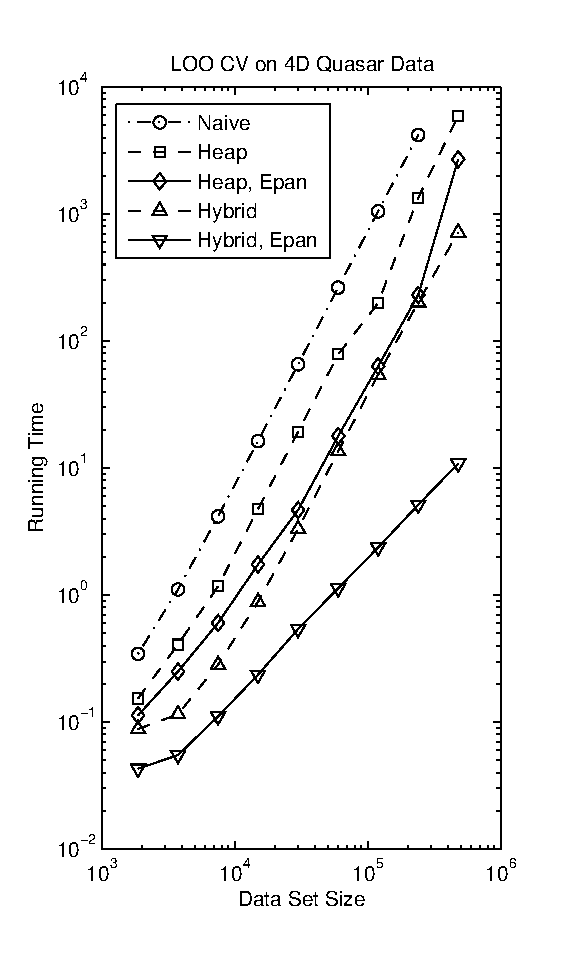
\includegraphics[width=3.1in]{quasar_times_narrow.eps}
  \end{center}
  \vspace{-30pt}
  \caption{\label{fig:quasar-speed}\footnotesize Running times for the
    na\"{i}ve algorithm, the algorithm from \cite{nbc-compstat}
    (heap), the improved expansion pattern (hybrid) and pruning
    opportunities (Epan) separately, and finally the improvements
    together.  Bandwidths were determined to maximize classification
    accuracy on the largest set and scaled via the theoretic inverse
    relationship to $N^{\frac{1}{5}}$.  Only one processor used.}
\end{figure}

\if 0
\begin{table}[b]
  \begin{center}\begin{tabular}{|l|r|r|r|r|r|r|r|r|r|}
    \hline
    \hline
    Size & 1875 & 3750 & 7500 & 15000 \\
    \hline
    \hline
    d \\
    \hline
    b \\
    \hline
    d \\
    \hline
    b \\
    \hline
    d \\
    \hline
    \hline
    30000 & 60000 & 120000 & 240000 & 480000 \\
    \hline
    \hline
    d \\
    \hline
    b \\
    \hline
    d \\
    \hline
    b \\
    \hline
    d \\
    \hline
    \hline
  \end{tabular}\end{center}\vspace{}
  \caption{Bob}
\end{table}
\fi

Three multi-bandwidth runs with 10 bandwidths per class, successively
narrowing the tested bandwidth ranges about the optimum, take 334,
127, and 86 seconds when parallelized over two processors.  Decreasing
running time is expected both because bandwidths are easier to prune
together if they are more similar to each other and because larger
bandwidths, which diminish as ranges tighten, tend to prune the least.
Figure~\ref{fig:multi-speed} demonstrates that the multi-bandwidth
algorithm is indeed much faster for a small number of bandwidths,
which is all that is necessary for optimization.  In comparison, the
estimated na\"{\i}ve running time for the above procedure is 140 hours
even if the algorithm utilizes the same density-sharing technique
employed by the multi-bandwidth algorithm.  Optimal bandwidths yield
within-class of accuracies of 95\% for quasars and 98\% for stars.

\begin{figure}[tb]
  \begin{center}
    \hspace*{-.3in}
    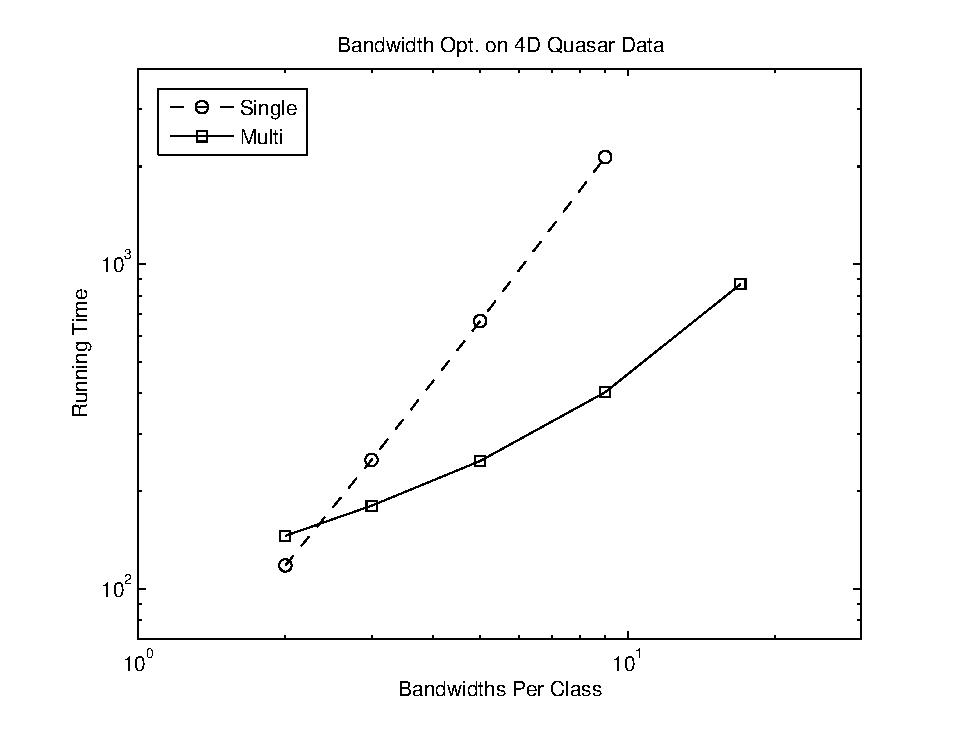
\includegraphics[width=3.6in]{multi_speed.eps}
    \hspace*{-.3in}
  \end{center}
  \vspace{-17pt}
  \caption{\label{fig:multi-speed}\footnotesize Running times for the
    multi-bandwidth algorithm and the single-bandwidth algorithm run
    on all bandwidth combinations.  Bandwidth range is constant
    between runs and bandwidths are tested at linear intervals.  Only
    one processor used.}
\end{figure}

Finally, we parallelize over multiple computers to tackle
classification of the full data set.  Using the a cosmologically
informed prior of 4\% for the quasar class, three dual-processor
machines discover just shy of one million quasars in 456 seconds.
Unfortunately, our parallelization methods see poor speed-up due to
serial data access and tree building, as shown in
Figure~\ref{fig:bad-para-speedup}.  These steps alone take about 310
seconds, the better portion of computation; the whole serial
computation takes only 640 seconds.  An important future avenue of
research is parallelizing tree building, but at current we are forced
to conclude that parallelization is not worthwhile at this scale.  In
any case, we far improve upon both the estimated na\"{\i}ve running
time of 380 hours, not to mention classifying the entire unknown data
a tenth the time it takes the old algorithm to test one bandwidth
combination.

\begin{figure}[tb]
  \begin{center}
    \hspace*{-.3in}
    \includegraphics[width=3.6in]{para_speedup.eps}
    \hspace*{-.3in}
  \end{center}
  \vspace{-15pt}
  \caption{\label{fig:bad-para-speedup}\footnotesize Speed-up for
    parallelized classification of the full 40m SDSS data set.
    Excluding data access and tree building shows that the underlying
    computation has workable speed-up.}
\end{figure}

Using careful tuning of parameters and separate classifiers for
separate regions of data, our collaborators have extracted more than
one million quasars from the SDSS data.  Hand-verification of subsets
of this data predicts that identified quasars are 85.6\% accurate and,
further, that we have identified 93.4\% of the quasars to be found.

\subsection{Forest Cover-Type Data.}
Originally used in \cite{blackard98}, the forest cover-type data is a
55-dimensional (10 continuous, 44 binary, 1 nominal classification)
data set with 580k observations describing the relationship between
cartographic variables and seven classes of forest cover-type,
i.e.~what kind of trees grow there.  Because KDA is not particularly
good at qualitative features (these would require scaling or a
specialized kernel), some preprocessing is required.  We normalize
each dimension to have unit variance and then perform PCA to reduce
the dimensionality to 8.  Further, as implemented, our algorithm only
supports two-class problems, so we will train our classifiers to
distinguish the one class from the rest of the data; results are shown
for distinguishing the largest class, lodgepole pines, which
constitutes nearly half of the data, and the smallest class,
cottonwoods and willows, which constitutes only 0.5\% of the data.

For lodgepole pines, we optimized bandwidths with three 10-by-10 runs
of the multi-bandwidth algorithm, taking 609, 135, and 92 seconds when
parallelized over two-processors.  The resulting classification
accuracy is 90\% both within and outside the class.  For cottonwoods
and willows, the same optimization procedure takes 1037, 248, and 213
seconds and result in a within-class accuracy of 99.4\% and 97.7\%
outside.  The estimated running time of the na\"{\i}ve algorithm for a
single bandwidth combination for the identification of either class is
10.6 hours, suggesting an overall time commitment of 320 hours for the
above work, around seven orders of magnitude slower.

Parallelization of LOO CV with the multi-bandwidth algorithm was much
more favorable than with the large SDSS query set.
Figure~\ref{fig:good-para-speedup} shows workable speed-up, suggesting
that iterations of the multi-bandwidth algorithm, especially the
long-running ones seen at higher dimensions, can still benefit greatly
from this extension.

\begin{figure}
  \begin{center}
    \hspace*{-.3in}
    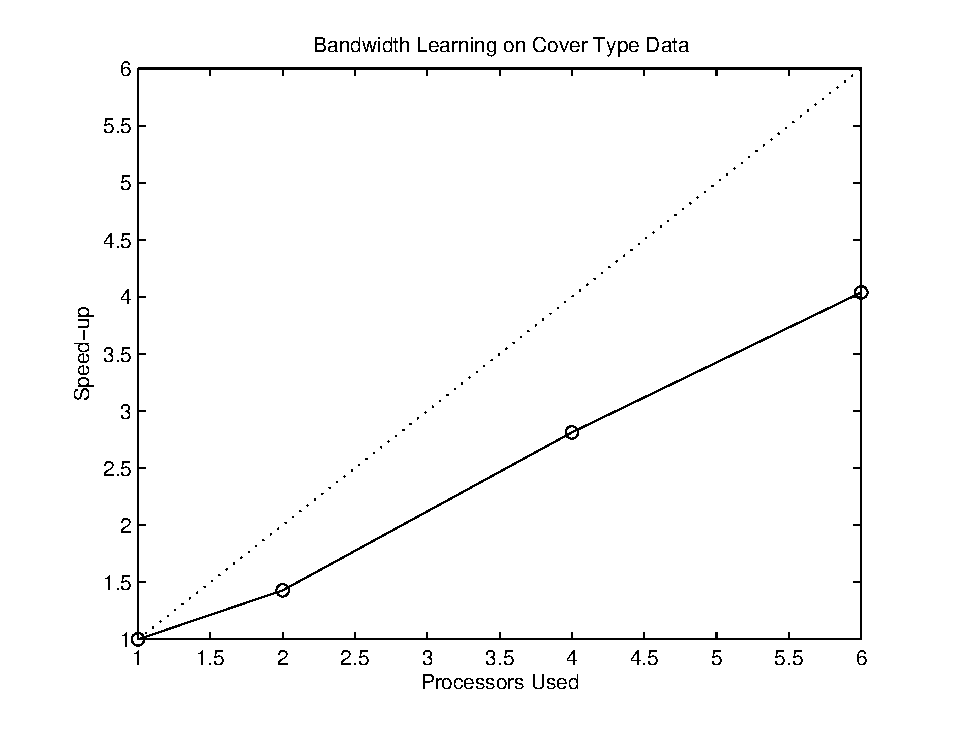
\includegraphics[width=3.6in]{covtype_speedup.eps}
    \hspace*{-.3in}
  \end{center}
  \vspace{-15pt}
  \caption{\label{fig:good-para-speedup}\footnotesize Speed-up for
    parallelized classification of LOO CV with the multi-bandwidth
    algorithm.}
\end{figure}

%\subsection{Synthetic Data.}

\section{Conclusion}
We have demonstrated numerous enhancements to the previous best
algorithm for KDA.  The hybrid expansion pattern and
inclusion/exclusion pruning have resulted in very clear gains in
asymptotic running time.  Further, the multi-bandwidth version of the
algorithm and parallelization enables rapid bandwidth learning for use
in classification or determination of accurate class probabilities.
We have significantly extended the size of problems now tractable
under this analysis, arriving at results in minutes where previously
it would have taken weeks.

Our algorithm's orders of magnitude speed-up is obtained with a
minimal degree of parallelization.  Through the use of a more advanced
data distribution and tree building method, we can expect
parallelization to yield even more impressive gains.  Also, as for
higher-dimensional problems, techniques such as logistic regression
may be used in combination with KDA, as in \cite{gray-highdimensional}.

Already, an earlier rendition of our quasar catalog has been used to
confirm the cosmic magnification effect predicted by the theory of
relativity \cite{nature05}.  The new, larger catalog that we have
found will undoubtedly lead to many other impressive discoveries.
Nonetheless, these are results from one data set in one scientific
application.  KDA has no special dependence upon quasar
identification, and in fact, the general methods \cite{nips2000paper}
behind our fast algorithm have no special dependence on KDA.  Methods
like those demonstrated in this paper have potential to accelerate a
wide variety of computations across science and data mining.

\begin{figure}[tb]
  \begin{center}\fbox{\begin{minipage}{3.1in}\vspace{-10pt}
  \begin{displaymath}\begin{array}{l}
    \xinit X = \kdroot{X},\:{\rm work} = \{\kdroot{Z_{1,2}}\} \\
    \xinit \vec{W}_{1,2} = 0,\:\vec{S}_{1,2} = 0,\:\vec{T}_{1,2} = 0 \\
    \xfunction \multi(X,{\rm work},\vec{W}_{1,2},\vec{S}_{1,2},\vec{T}_{1,2})
    \x \xinit \lo{\vec{\Phi}_1} = 0,\:\hi{\vec{\Phi}_1} = 0,\:\lo{\vec{\Phi}_2} = 0,\:\hi{\vec{\Phi}_2} = 0
    \x \xinit {\rm next} \text{ to be empty}
    \x \xfor \xeach Z_{1,2} \in {\rm work}
    \xx \xfor i \text{ from } {\rm hi}(Z_1) \text{ to } {\rm lo}(Z_1)
    \xxx \xif \hi{d}(X,Z_1) \leq h_1^i
    \xxxx \vec{W}_1{\scriptstyle \!(i)} \peq W(Z_1)
    \xxxx \text{... // Similar for $\vec{S}_1$ and $\vec{T}_1$}
%    \xxxx \vec{S}_1{\scriptstyle \!(i)} \peq S(Z_1)
%    \xxxx \vec{T}_1{\scriptstyle \!(i)} \peq T(Z_1)
    \xxx \xelse \xbreak
    \xx \xfor i \text{ continuing to } {\rm lo}(Z_1)
    \xxx \xif \lo{d}(X,Z_1) < h_1^i,
    \xxxx \lo{\vec{\Phi}_1}{\scriptstyle \!(i)} \peq W(Z_1) K_{h_1^i}(\hi{d}(X,Z_1))
    \xxxx \hi{\vec{\Phi}_1}{\scriptstyle \!(i)} \peq W(Z_1) K_{h_1^i}(\lo{d}(X,Z_1))
    \xxx \xelse \xbreak
    \xx \text{update ${\rm lo}(Z_1)$ and ${\rm hi}(Z_1)$}
    \xx \text{... // Similar for $Z_2$}
%    \xx \xfor j \text{ from } {\rm hi}(Z_2) \text{ to } {\rm lo}(Z_2)
%    \xxx \xif \hi{d}(X,Z_2) \leq h_2^j
%    \xxxx \vec{W}_2{\scriptstyle \!(j)} \peq W(Z_2)
%    \xxxx \text{... // Similar for $\vec{S}_2$ and $\vec{T}_2$}
%%    \xxxx \vec{S}_2{\scriptstyle \!(j)} \peq S(Z_2)
%%    \xxxx \vec{T}_2{\scriptstyle \!(j)} \peq T(Z_2)
%    \xxx \xelse \xbreak
%    \xx {\rm hi}(Z_2) = j
%    \xx \xfor j \text{ continuing to } {\rm lo}(Z_2)
%    \xxx \xif \lo{d}(X,Z_2) < h_2^j,
%    \xxxx \lo{\vec{\Phi}_2}{\scriptstyle \!(j)} \peq W(Z_2) K_{h_2^j}(\hi{d}(X,Z_2))
%    \xxxx \hi{\vec{\Phi}_2}{\scriptstyle \!(j)} \peq W(Z_2) K_{h_2^j}(\lo{d}(X,Z_2))
%    \xxx \xelse \xbreak
%    \xx {\rm lo}(Z_2) = j+1
    \xx \xif {\rm lo}(Z_1) \leq {\rm hi}(Z_1) \text{ or } {\rm lo}(Z_2) \leq {\rm hi}(Z_2)
    \xxx \text{add $\kdleft{Z}$ and $\kdright{Z}$ to } {\rm next}
    \x \xfor i \text{ from } {\rm lo}_1(X) \text{ to } {\rm hi}_1(X)
    \xx \lo{\vec{\Phi}_1}{\scriptstyle \!(i)} \peq \vec{W}_1{\scriptstyle \!(i)} K_{h_1^i}(\hi{\delta}(X,\vec{W}_1{\scriptstyle \!(i)},\vec{S}_1{\scriptstyle \!(i)},\vec{T}_1{\scriptstyle \!(i)}))
    \xx \hi{\vec{\Phi}_1}{\scriptstyle \!(i)} \peq W_1{\scriptstyle \!(i)} K_{h_1^i}(\lo{\delta}(X,W_1{\scriptstyle \!(i)},S_1{\scriptstyle \!(i)},T_1{\scriptstyle \!(i)}))
    \x \text{... // Similar for $\lo{\vec{\Phi}_2}$ and $\hi{\vec{\Phi}_2}$}
%    \x \xfor j \text{ from } {\rm lo}_2(X) \text{ to } {\rm hi}_2(X)
%    \xx \lo{\vec{\Phi}_2}{\scriptstyle \!(j)} \peq \vec{W}_2{\scriptstyle \!(j)} K_{h_2^j}(\hi{\delta}(X,\vec{W}_2{\scriptstyle \!(j)},\vec{S}_2{\scriptstyle \!(j)},\vec{T}_2{\scriptstyle \!(j)}))
%    \xx \hi{\vec{\Phi}_2}{\scriptstyle \!(j)} \peq W_2{\scriptstyle \!(j)} K_{h_2^j}(\lo{\delta}(X,W_2{\scriptstyle \!(j)},S_2{\scriptstyle \!(j)},T_2{\scriptstyle \!(j)}))
    \x \xfor i \text{ from } {\rm lo}_1(X) \text{ to } {\rm hi}_1(X)
    \xx \xfor j \text{ from } {\rm lo}_2(X) \text{ to } {\rm hi}_2(X)
    \xxx \xif (1-t) \lo{\vec{\Phi}_1}{\scriptstyle \!(i)} \lo{\Pi}(X) > t \hi{\vec{\Phi}_2}{\scriptstyle \!(j)} (1 - \lo{\Pi}(X)),
    \xxxx \text{label $X$ as $C_1$ for $(i,j)$}
    \xxx \xif t \lo{\vec{\Phi}_2}{\scriptstyle \!(j)} (1 - \hi{\Pi}(X)) > (1-t) \hi{\vec{\Phi}_1}{\scriptstyle \!(i)} \hi{\Pi}(X),
    \xxxx \text{label $X$ as $C_2$ for $(i,j)$}
    \x \text{update ${\rm lo}_1(X)$, ${\rm hi}_1(X)$, ${\rm lo}_2(X)$, and ${\rm hi}_2(X)$}
    \x \xif {\rm lo}_1(X) \leq {\rm hi}_1(X) \text{ and } {\rm lo}_2(X) \leq {\rm hi}_2(X)
    \xx \multi(\kdleft{X},{\rm next},\vec{W}_{1,2},\vec{S}_{1,2},\vec{T}_{1,2})
    \xx \multi(\kdright{X},{\rm next},\vec{W}_{1,2},\vec{S}_{1,2},\vec{T}_{1,2})
  \end{array}\end{displaymath}
  \end{minipage}}\end{center}
  \vspace{-10pt}
  \caption{\label{fig:multi} \footnotesize Pseudocode for the
    multi-bandwidth algorithm.  For either class, the algorithm checks
    for and handles inclusion prunes followed by normal bounds
    computations until the first exclusion prune.  Pruned
    contributions are then applied for each bandwidth and bandwidth
    combinations are tested for classification.  Handling of base-case
    omitted.}
\end{figure}

\bibliographystyle{abbrv}
\bibliography{nbc_siam07}

\end{document}
